\documentclass[12pt]{article}

\usepackage{fullpage}
\usepackage{mdframed}
\usepackage{colonequals}
\usepackage{algpseudocode}
\usepackage{algorithm}
\usepackage{tcolorbox}
\usepackage[all]{xy}
\usepackage{proof}
\usepackage{mathtools}
\usepackage{bbm}
\usepackage{amssymb}
\usepackage{amsthm}
\usepackage{amsmath}
\usepackage{amsxtra}
\newcommand{\bb}{\mathbb}


\newtheorem{theorem}{Theorem}[section]
\newtheorem{corollary}{Corollary}[theorem]
\newtheorem{lemma}{Lemma}

\newcommand{\mathcat}[1]{\textup{\textbf{\textsf{#1}}}} % for defined terms

\newenvironment{problem}[1]
{\begin{tcolorbox}\noindent\textbf{Problem #1}.}
{\vskip 6pt \end{tcolorbox}}

\newenvironment{enumalph}
{\begin{enumerate}\renewcommand{\labelenumi}{\textnormal{(\alph{enumi})}}}
{\end{enumerate}}

\newenvironment{enumroman}
{\begin{enumerate}\renewcommand{\labelenumi}{\textnormal{(\roman{enumi})}}}
{\end{enumerate}}

\newcommand{\defi}[1]{\textsf{#1}} % for defined terms

\theoremstyle{remark}
\newtheorem*{solution}{Solution}

\setlength{\hfuzz}{4pt}

\newcommand{\calC}{\mathcal{C}}
\newcommand{\calF}{\mathcal{F}}
\newcommand{\C}{\mathbb C}
\newcommand{\N}{\mathbb N}
\newcommand{\Q}{\mathbb Q}
\newcommand{\R}{\mathbb R}
\newcommand{\Z}{\mathbb Z}
\newcommand{\br}{\mathbf{r}}
\newcommand{\RP}{\mathbb{RP}}
\newcommand{\CP}{\mathbb{CP}}
\newcommand{\nbit}[1]{\{0, 1\}^{#1}}
\newcommand{\bits}{\{0, 1\}^{n}}
\newcommand{\bbni}{\bigbreak \noindent}
\newcommand{\norm}[1]{\left\vert\left\vert#1\right\vert\right\vert}

\let\1\relax
\newcommand{\1}{\mathbf{1}}
\newcommand{\fr}[2]{\left(\frac{#1}{#2}\right)}

\newcommand{\vecz}{\mathbf{z}}
\newcommand{\vecr}{\mathbf{r}}
\DeclareMathOperator{\Cinf}{C^{\infty}}
\DeclareMathOperator{\Id}{Id}

\DeclareMathOperator{\Alt}{Alt}
\DeclareMathOperator{\ann}{ann}
\DeclareMathOperator{\codim}{codim}
\DeclareMathOperator{\End}{End}
\DeclareMathOperator{\Hom}{Hom}
\DeclareMathOperator{\id}{id}
\DeclareMathOperator{\M}{M}
\DeclareMathOperator{\Mat}{Mat}
\DeclareMathOperator{\Ob}{Ob}
\DeclareMathOperator{\opchar}{char}
\DeclareMathOperator{\opspan}{span}
\DeclareMathOperator{\rk}{rk}
\DeclareMathOperator{\sgn}{sgn}
\DeclareMathOperator{\Sym}{Sym}
\DeclareMathOperator{\tr}{tr}
\DeclareMathOperator{\img}{img}
\DeclareMathOperator{\CandE}{CandE}
\DeclareMathOperator{\CandO}{CandO}
\DeclareMathOperator{\argmax}{argmax}
\DeclareMathOperator{\first}{first}
\DeclareMathOperator{\last}{last}
\DeclareMathOperator{\cost}{cost}
\DeclareMathOperator{\dist}{dist}
\DeclareMathOperator{\path}{path}
\DeclareMathOperator{\parent}{parent}
\DeclareMathOperator{\argmin}{argmin}
\DeclareMathOperator{\excess}{excess}
\let\Pr\relax
\DeclareMathOperator{\Pr}{\mathbf{Pr}}
\DeclareMathOperator{\Exp}{\mathbb{E}}
\DeclareMathOperator{\Var}{\mathbf{Var}}
\let\limsup\relax
\DeclareMathOperator{\limsup}{limsup}
%Paired Delims
\DeclarePairedDelimiter\ceil{\lceil}{\rceil}
\DeclarePairedDelimiter\floor{\lfloor}{ \rfloor}


\newcommand{\dagstar}{*}

\newcommand{\tbigwedge}{{\textstyle{\bigwedge}}}
\setlength{\parindent}{0pt}
\setlength{\parskip}{5pt}


\begin{document}

\title{CS 40: Computational Complexity}

\author{Sair Shaikh}
\maketitle

% Collaboration Notice: Talked to Henry Scheible '26 to discuss ideas.



\begin{problem}{1}(2.3.1) \\
    If $T_n(X,A)$ denotes the torsion subgroup of $H_n(X,A)$, show that the functors $(X,A) \mapsto T_n(X,A)$ with the obvious induced homomorphisms $T_n(X,A) \to T_n(Y,B)$ and boundary maps $T_n(X,A) \to T_{n-1}(A)$ do not satisfy a homology theory even if excluding the dimension axiom. Do the same for the `mod-torsion' functor $MT_n(X,A) = H_n(X,A)/T_n(X,A)$. 
\end{problem}

\begin{solution}
    We will show a contradiction to the exactness axiom. Let $X$ be the Mobius strip and $A$ be the boundary circle of the Mobius strip. Then, we must have the long exact sequence: 
    \[\cdots \to H_1(A) \to H_1(X) \to H_1(X, A) \to H_0(A) \to H_0(X) \to  \cdots \]
    Let $C$ be the center circle. We showed in Hwk 3, Problem 3.3, that $X$ deformation retracts to $C$ via the straight-line homotopy (this is also clear from the CW complex picture). Thus, $\pi_1(X) \cong \pi_1(C) = \Z$. Since $H_1$ is the abelianization of $\pi_1$, we have $H_1(X) \cong \Z$. \bbni 
    Moreover, $H_1(A) \cong \Z$ as well, since $A$ is a circle. Moreover, note that we showed (in Hwk 3, Problem 3.3) that the generator for $H_1(A)$, i.e. the loop around $A$ maps to $2$ times the generator of $H_1(C)$, thus maps to $2$ times the generator of $H_1(X)$ (as deformation retraction is a homotopy equivalence, thus isomorphism on the homology). \bbni
    Finally, we have that $H_0(A) \cong H_0(X) \cong \Z$ and the pushforward of the inclusion map on $H_0$ is an isomorphism as the spaces are path-connected. Thus, we get: 
    \[\cdots \to \Z \xrightarrow{2} \Z \to H_1(X, A) \to \Z \xrightarrow{\sim} \Z \to \cdots \]
    Then, the kernel of the second map is the image of the first map, i.e. $2\Z$. Thus, the image of the second map is $\cong \Z/2\Z$ (first isomorphism theorem). Thus, we have that $\ker(H_1(X, A) \to \Z) \cong \Z/2\Z$. \\
    Moreover, the last map is an isomormphism, hence injective, thus the map $H_1(X, A) \to \Z$ is $0$. Thus, the kernel is everything, i.e. $H_1(X, A) \cong \Z/2\Z$. Thus, our long exact sequence becomess:
    \[ \cdots \to \Z \xrightarrow{2} \Z \to \Z/2\Z \to 0 \to \cdots \]
    Applying the torsion functor $T$, we have: 
    \begin{align*}
        \cdots \to \underbrace{0}_{T_1(A)} \to \underbrace{0}_{T_1(X)} \to \underbrace{\Z/2\Z}_{T_1(X,A)} \to 0 \to \cdots
    \end{align*}
    is not exact (the boundary maps are the natural ones from functoriality) as the image of the second map is trivial, but the kernel of the third map is $\Z/2\Z$. Thus, $T$ fails the exactness axiom. \bbni 
    Similarly, applying the mod-torsion functor $MT$, we have: 
    \begin{align*}
        \cdots \to \underbrace{\Z}_{MT_1(A)} \xrightarrow{2} \underbrace{\Z}_{MT_1(X)} \to \underbrace{0}_{MT_1(X,A)} \to 0 \to \cdots
    \end{align*}
    (the $2$ map is preserved as be modded nothing out). Again, this is not exact at $MT_1(X)$ as the image of the first map is $2\Z$ while the kernel of the second map is $\Z$. Thus, the mod-torsion functor does not satisfy the exactness axiom. \bbni
\end{solution}
\newpage

\begin{problem}{2}(2.3.5, with $G= \Z$) 
    Regarding a cochain $\varphi \in C^1(X)$ as a function on paths in $X$ to $\Z$, show that if $\varphi$ is a cocycle, then 
    \begin{enumerate}
    \item $\varphi(f \cdot g) = \varphi(f) + \varphi(g)$,
    \item $\varphi$ takes the value $0$ on constant paths,
    \item $\varphi(f) = \varphi(g)$ if $f \simeq_p g$, and
    \item $\varphi$ is a coboundary if and only if $\varphi(f)$ depends only on the endpoints of $f$ for all paths $f$ in $X$.
    \end{enumerate}
\end{problem}

\begin{solution}
    \bbni
    \begin{enumerate}
        \item Recall that a cochain $\varphi \in C^1(X)$ is a cocycle if $\delta \varphi = 0$. However, we have, by definition, for $\sigma: \Delta^2 \to X$ that: 
        \[ \delta(\varphi)(\sigma) = \varphi(\delta \sigma) = 0\]
        Thus, $\varphi$ is $0$ on all boundaries. \bbni
        We construct $\sigma: \Delta^2 \to X$ with sides $[v_1, v_2] = f$, $[v_2, v_3] = g$ and $[v_1, v_3] = f \cdot g$ as follows: \bbni
        \begin{centering}
            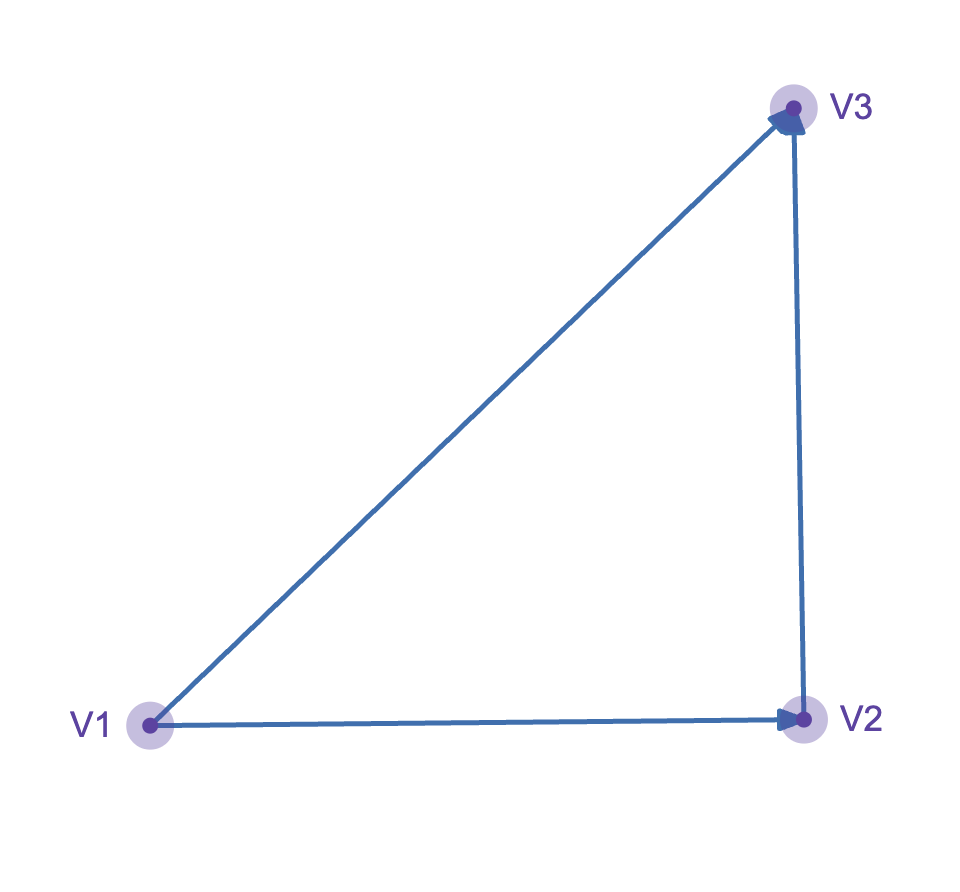
\includegraphics[width=0.5\textwidth]{assets/hwk9_21.png}
        \end{centering}
        \bbni
        Then, we have: 
        \begin{align*}
            \varphi(\delta \sigma) &= \varphi(g) - \varphi(f \cdot g) + \varphi(f) = 0
        \end{align*}
        Thus, we have $\varphi(f \cdot g) = \varphi(f) + \varphi(g)$.
        \item Let $\id_e$ be the constant path at point $e \in X$. The constant path is the boundary of the 2-simplex $\sigma: \Delta^2 \to X$ with all vertices mapped to $e$ (thus all edges constant paths $\id_{e}$). Then, we have:
        \begin{align*}
            \varphi(\delta \sigma) &= \varphi(\id_e) - \varphi(\id_e) + \varphi(\id_e) = 0
        \end{align*}
        Thus, $\varphi(\id_e) = 0$.
        \item If $f \simeq_p g$ are paths from $x_0$ to $x_1$, then we can construct two $2$-simplices as in the diagram: \bbni
        \begin{centering}
            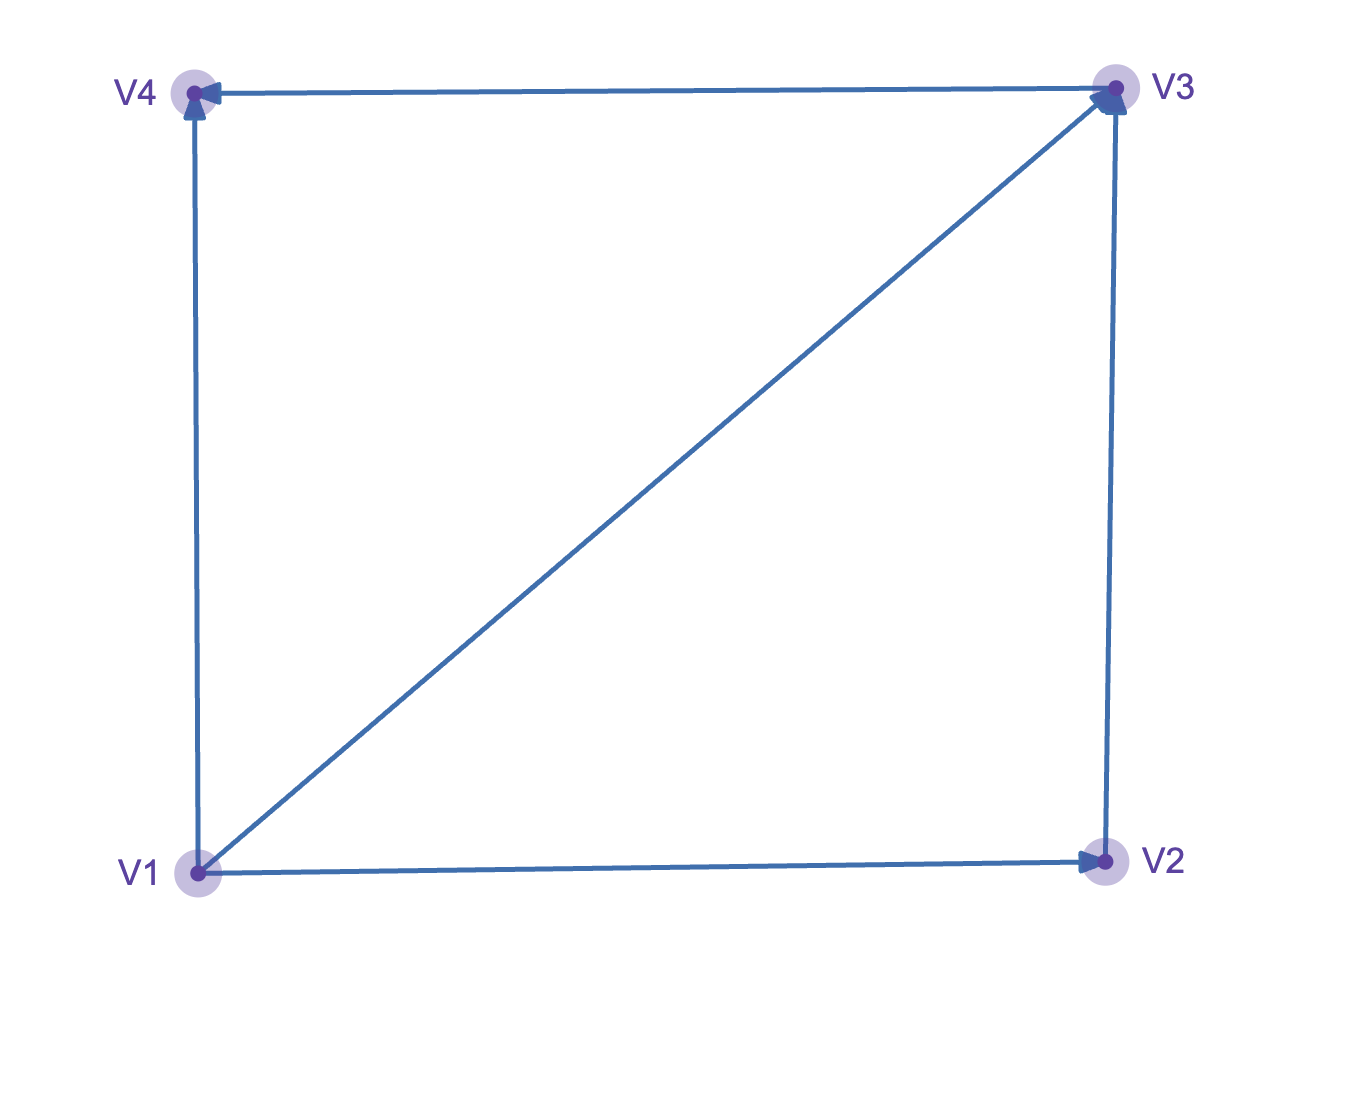
\includegraphics[width=0.5\textwidth]{assets/hwk9_22.png}
        \end{centering}    
        \bbni   
        with $[v_1, v_2] = f$, $[v_1, v_3] = \psi$, $[v_1, v_4] = id_{x_0}$, $[v_2, v_3] = \id_{x_1}$, and $[v_3, v_4] = -g$. Then, we have: 
        Then, we have:
        \begin{align*}
            \varphi(\delta (\sigma_1 + \sigma_2)) &= \varphi([v_2, v_3]) - \varphi([v_1, v_3]) + \varphi([v_1, v_3]) + \varphi([v_3, v_4]) - \varphi([v_1, v_4]) + \varphi([v_1, v_3]) \\
            &= \varphi(\id_{x_1}) - \varphi(\psi) + \varphi(f) + \varphi(-g) - \varphi(\id_{x_0}) +  \varphi(\psi) \\
            &= \varphi(f) - \varphi(g) \\
            &= 0
        \end{align*}
        Thus, 
        \begin{align*}
            \varphi(f) &= \varphi(g)
        \end{align*}
        Note that I assumed $\varphi(-g) = -\varphi(g)$, which can be avoided by swapping $v_3$ and $v_4$ and just having $[v_3, v_4] = g$, but also, we implicitly use $[v_i, v_j] = -[v_j, v_i]$ often. \bbni 
        Note that also these three parts together imply that $\varphi(f^{-1}) = -\varphi(f)$, since $f \cdot f^{-1} \simeq_p \id_{x_0}$, and then $\varphi(f^{-1}) + \varphi(f) = \varphi(\id_{x_0}) = 0$, where $x_0$ is the start point of $f$.
        \item If $\varphi$ is a coboundary there exists a $0$-cochain $\psi \in C^0(X)$ such that $\varphi = \delta \psi$. Thus, for $f: \Delta^1 \to X$ with endpoints $x_0$ and $x_1$, we have:
        \begin{align*}
            \varphi(f) &= \delta \psi(f) \\
            &= \psi(\delta f) \\
            &= \psi(x_1) - \psi(x_0)
        \end{align*}
        Thus, $\varphi(f)$ depends only on the endpoints of $f$. \bbni
        Conversely, assume $\varphi(f)$ depends only on the endpoints of $f$. Let $X'$ be a path-connected component. Pick a basepoint $x \in X'$. Then, for any $x' \in X'$, we can construct a path $f_{x'}: \Delta^1 \to X'$ from $x$ to $x'$. Then, we define $\psi: X' \to \Z$ by:
        \[ \psi(x') := \varphi(f_{x'})\]
        since $\varphi(f)$ depends only on the endpoints, this is well-defined. Similarly, we do this for all path-connected components of $X$. Then, if $f$ is a path from $x_0$ to $x_1$ in path-connected component with basepoint $x$, we construct $f_1$ and $f_2$, paths from $x$ to $x_1$ and $x_2$, respectively. Then, we have:
        \begin{align*}
            \varphi(f) &= \varphi(f_1^{-1} \cdot f_2) \\
            &= -\varphi(f_1) + \varphi(f_2) \\
            &= -\psi(x_1) + \psi(x_2) \\
            &= \psi(\delta f) \\
            &= \delta \psi(f)
        \end{align*}
        Thus, $\varphi$ is a coboundary.
    \end{enumerate}
\end{solution}
\newpage

\begin{problem}{3}
Verify the remark in Hatcher after exercise 2.3.5: If $X$ is path-connected, the previous problem together with the universal coefficient theorem induces an isomorphism $H^1(X) \cong \mathrm{Hom}(\pi_1(X), \Z)$.
\end{problem}
\begin{solution}
    We calculate $Ext^1(H_0(X), \Z)$. This represents the isomorphism classes of extensions: 
    \[ 0 \to \Z \to A \to H_0(X) \to 0 \]
    Since $X$ is path-connected, we have $H_0(X) \cong \Z$. Thus, there are no extensions and $Ext^1(H_0(X), \Z) = 0$. Then, note the universal coefficient theorem gives us the exact sequence: 
    \[ 0 \to H^1(X) \to \Hom(H_1(X), \Z) \to 0 \]
    Thus, we have $H^1(X) \cong \Hom(H_1(X), \Z)$. \bbni
    Define $\Phi: Z^1(X) \to \Hom(\pi_1(X), \Z)$ as follows:
    \[ \Phi(\varphi)([\gamma]) = \varphi(\gamma) \]
    where $\varphi \in Z^1(X)$ is a cocycle and $[\gamma] \in \pi_1(X)$. This is well-defined by part (3), and a homomorphism by part (1) and (2) of the previous problem. We claim that $\Phi$ is surjective. \bbni
    Let $\rho: \pi_1(X) \to \Z$ be a homomorphism. We define a cocycle $\varphi \in Z^1(X)$ for path $f$ from $x_1$ to $x_2$ as follows. Let $\alpha_{x_1}, \alpha_{v_2}$ be paths from $x_0$ (the basepoint of $\pi_1(X)$) to $x_1$ and $x_2$, respectively. Then, we define:
    \[ \varphi(f) = \rho([\alpha_{x_1} \cdot f \cdot \alpha_{x_2}^{-1}]) \]
    One can verify this is a cocycle. Let $\sigma: \Delta^2 \to X$ be a $2$-simplex with sides $[v_1, v_2]$, $[v_2, v_3]$ and $[v_3, v_1]$. Then, 
    \begin{align*}
        \varphi(\delta \sigma) &= \rho([\alpha_{v_2} \cdot [v_2, v_3] \cdot \alpha_{v_3}^{-1}]) - \rho([\alpha_{v_1} \cdot [v_1, v_3] \cdot \alpha_{v_3}^{-1}])+ \rho([\alpha_{v_1} \cdot [v_1, v_2] \cdot \alpha_{v_2}^{-1}]) \\
        &= \rho([\alpha_{v_2} \cdot [v_2, v_3] \cdot \alpha_{v_3}^{-1} \cdot \alpha_{v_3} \cdot [v_3, v_1] \cdot \alpha_{v_1}^{-1} \cdot \alpha_{v_1} \cdot [v_1, v_2] \cdot \alpha_{v_2}^{-1}])\\
        &= \rho([\alpha_{v_2} \cdot [v_2, v_3] \cdot [v_3, v_1] \cdot [v_1, v_2] \cdot \alpha_{v_2}^{-1}])\\
        &= \rho([\alpha_{v_2} \cdot \id_{v_2} \cdot \alpha_{v_2}^{-1}])\\
        &= \rho(\id_{v_2}) = 0
    \end{align*}
    Thus, $\varphi$ is a cocycle and $\Phi$ is surjective. \bbni
    Next, we investigate $\ker(\Phi)$. Assume $\Phi(\varphi) = 0$. Then $\varphi(\gamma) = 0$ for all $\gamma \in \pi_1(X)$. Then, $\varphi$ trivially depends only on the endpoints of $\gamma$, thus is a coboundary by part (4) of the previous problem. Thus, $\ker(\Phi) \subseteq B^1(X)$. Moreover, if $\varphi$ is a coboundary, it depends only on the endpoints of any path. Thus, as paths in $\pi_1(X)$ are loops, $\varphi$ is constant on $\pi_1(X)$. Thus, $\varphi(\gamma) = \varphi(\id) = 0$ for all $\gamma \in \pi_1(X)$. Thus, $B^1(X) \subseteq \ker(\Phi)$. Thus, $\ker(\Phi) = B^1(X)$. \bbni
    Then, by the first isomorphism theorem, we have:
    \[ H^1(X) = Z^1(X)/B^1(X) \cong \Hom(\pi_1(X), \Z) \]
\end{solution}
\newpage




\end{document}